\documentclass[border=8pt]{standalone}
\usepackage{amsmath,amssymb}
\usepackage[scaled]{helvet}                 % Arial-equivalent sans (OUP: sans-serif, prefer Arial)
\renewcommand{\familydefault}{\sfdefault}   % make sans the DEFAULT so \bfseries/\footnotesize stay sans
\usepackage{xcolor}
\usepackage{tikz}
\usetikzlibrary{arrows.meta,positioning,calc,fit,backgrounds,shapes.geometric}

% ---- macros (mirror supplement_engine_math.tex) ----
\newcommand{\REF}{\mathrm{REF}}
\newcommand{\HET}{\mathrm{HET}}
\newcommand{\ALT}{\mathrm{ALT}}
\newcommand{\BetaBin}{\mathrm{BetaBin}}

% ---- palette ----
\definecolor{stateblue}{HTML}{2F5FA8}
\definecolor{emitoch}{HTML}{C07A1E}
\definecolor{ink}{HTML}{2B333B}
\definecolor{softgray}{HTML}{6B7784}

\begin{document}
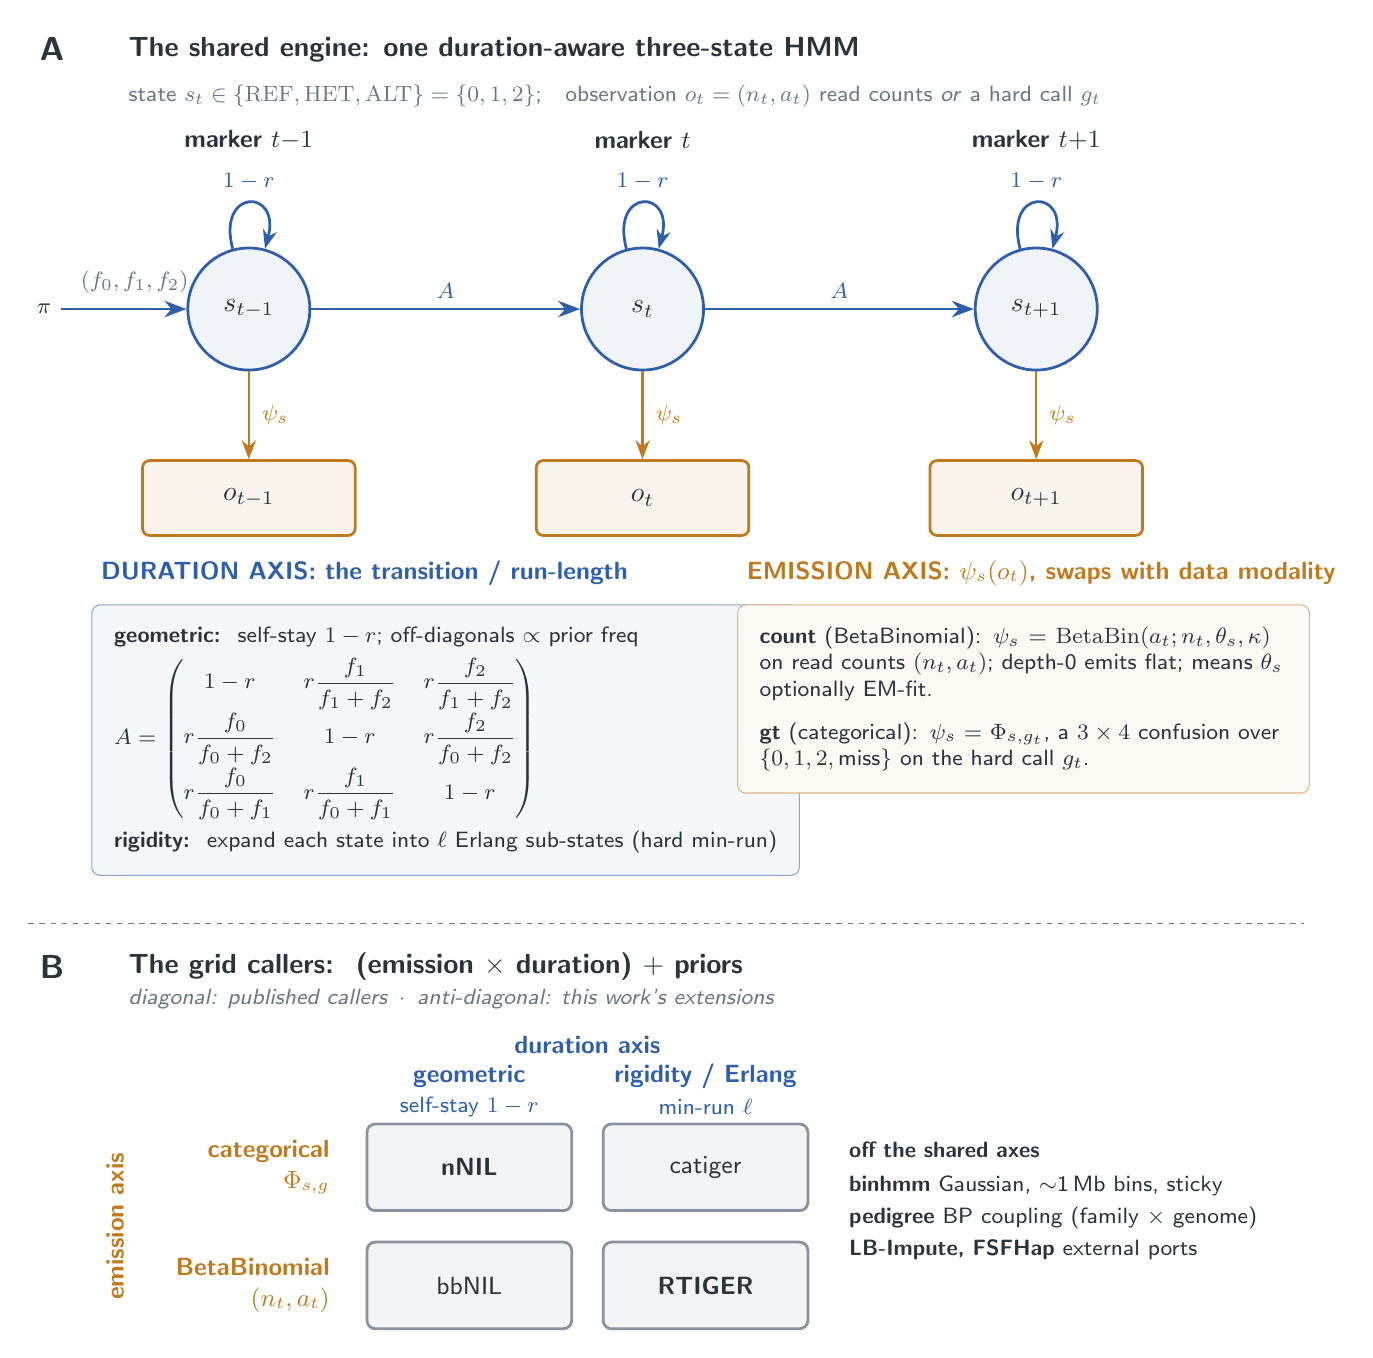
\begin{tikzpicture}[
  font=\sffamily,
  state/.style={circle, draw=stateblue, line width=1pt, fill=stateblue!7,
                minimum size=1.55cm, inner sep=0pt, text=ink},
  obs/.style={rounded corners=2.5pt, draw=emitoch, line width=1pt, fill=emitoch!8,
              minimum width=2.7cm, minimum height=0.95cm, align=center, text=ink},
  tarrow/.style={-{Stealth[length=2.8mm]}, line width=1pt, draw=stateblue},
  earrow/.style={-{Stealth[length=2.4mm]}, line width=0.9pt, draw=emitoch},
  selfloop/.style={-{Stealth[length=2.4mm]}, line width=1pt, draw=stateblue,
                   loop above, looseness=5, min distance=7mm},
  mlabel/.style={font=\small\bfseries, text=ink},
  boxhead/.style={font=\small\bfseries},
  matbox/.style={rounded corners=3pt, draw=stateblue!55, fill=stateblue!5,
                 inner sep=8pt, text=ink, align=left, font=\footnotesize},
  plabel/.style={font=\large\bfseries, text=ink},
]

% ============================================================= PANEL (a)
\node[plabel] at (-0.3,11.7) {A};
\node[font=\bfseries, text=ink, anchor=west] at (0.55,11.7)
   {The shared engine: one duration-aware three-state HMM};
\node[font=\footnotesize, text=softgray, anchor=west] at (0.55,11.1)
   {state $s_t\in\{\REF,\HET,\ALT\}=\{0,1,2\}$;\quad observation $o_t=(n_t,a_t)$ read counts \emph{or} a hard call $g_t$};

% marker column labels
\node[mlabel] at (2.2,10.55) {marker $t{-}1$};
\node[mlabel] at (7.2,10.55) {marker $t$};
\node[mlabel] at (12.2,10.55) {marker $t{+}1$};

% hidden states
\node[state] (s1) at (2.2,8.4) {$s_{t-1}$};
\node[state] (s2) at (7.2,8.4) {$s_t$};
\node[state] (s3) at (12.2,8.4) {$s_{t+1}$};

% initial
\node[font=\footnotesize, text=ink] (initlab) at (-0.4,8.4) {$\pi$};
\draw[tarrow] (initlab) -- (s1);
\node[font=\footnotesize, text=softgray] at (0.75,8.75) {$(f_0,f_1,f_2)$};

% self-loops (duration axis)
\draw[selfloop] (s1) to node[font=\footnotesize, text=stateblue, above=1pt] {$1-r$} (s1);
\draw[selfloop] (s2) to node[font=\footnotesize, text=stateblue, above=1pt] {$1-r$} (s2);
\draw[selfloop] (s3) to node[font=\footnotesize, text=stateblue, above=1pt] {$1-r$} (s3);

% transitions
\draw[tarrow] (s1) -- node[font=\footnotesize, text=stateblue, above] {$A$} (s2);
\draw[tarrow] (s2) -- node[font=\footnotesize, text=stateblue, above] {$A$} (s3);

% observations + emissions (emission axis)
\node[obs] (o1) at (2.2,6.0) {$o_{t-1}$};
\node[obs] (o2) at (7.2,6.0) {$o_{t}$};
\node[obs] (o3) at (12.2,6.0) {$o_{t+1}$};
\draw[earrow] (s1) -- node[font=\footnotesize, text=emitoch, right=1pt] {$\psi_s$} (o1);
\draw[earrow] (s2) -- node[font=\footnotesize, text=emitoch, right=1pt] {$\psi_s$} (o2);
\draw[earrow] (s3) -- node[font=\footnotesize, text=emitoch, right=1pt] {$\psi_s$} (o3);

% ---- DURATION AXIS module box ----
\node[boxhead, text=stateblue, anchor=west] at (0.2,5.05)
   {DURATION AXIS: the transition / run-length};
\node[matbox, anchor=north west] (Abox) at (0.2,4.65) {%
  \renewcommand{\arraystretch}{1.05}%
  \textbf{geometric:}\; self-stay $1-r$; off-diagonals $\propto$ prior freq\\[3pt]
  $A=\begin{pmatrix}
     1-r & r\dfrac{f_1}{f_1+f_2} & r\dfrac{f_2}{f_1+f_2}\\[6pt]
     r\dfrac{f_0}{f_0+f_2} & 1-r & r\dfrac{f_2}{f_0+f_2}\\[6pt]
     r\dfrac{f_0}{f_0+f_1} & r\dfrac{f_1}{f_0+f_1} & 1-r
   \end{pmatrix}$\\[3pt]
  \textbf{rigidity:}\; expand each state into $\ell$ Erlang sub-states (hard min-run)};

% ---- EMISSION AXIS module box ----
\node[boxhead, text=emitoch, anchor=west] at (8.4,5.05)
   {EMISSION AXIS: $\psi_s(o_t)$, swaps with data modality};
\node[matbox, draw=emitoch!55, fill=emitoch!5, anchor=north west, text width=6.7cm] (Ebox) at (8.4,4.65) {%
  \textbf{count} (BetaBinomial): $\psi_s=\BetaBin(a_t;n_t,\theta_s,\kappa)$ on read counts $(n_t,a_t)$; depth-0 emits flat; means $\theta_s$ optionally EM-fit.\\[6pt]
  \textbf{gt} (categorical): $\psi_s=\Phi_{s,g_t}$, a $3\times4$ confusion over $\{0,1,2,\text{miss}\}$ on the hard call $g_t$.};

% ============================================================= divider
\draw[softgray, line width=0.5pt, dash pattern=on 2pt off 2pt] (-0.6,0.6) -- (15.6,0.6);

% ============================================================= PANEL (b)
\node[plabel] at (-0.3,0.05) {B};
\node[font=\bfseries, text=ink, anchor=west] at (0.55,0.05)
   {The grid callers:\; (emission $\times$ duration) $+$ priors};
\node[font=\footnotesize\itshape, text=softgray, anchor=west] at (0.55,-0.36)
   {diagonal: published callers\, $\cdot$\, anti-diagonal: this work's extensions};

% grid geometry
\def\cLx{5.0}\def\cRx{8.0}          % column centers
\def\rTy{-2.5}\def\rBy{-4.0}        % row centers (top=categorical, bottom=BetaBinomial)

% duration-axis (columns)
\node[font=\small\bfseries, text=stateblue] at (6.5,-0.95) {duration axis};
\node[font=\small\bfseries, text=stateblue] at (\cLx,-1.35) {geometric};
\node[font=\small\bfseries, text=stateblue] at (\cRx,-1.35) {rigidity / Erlang};
\node[font=\footnotesize, text=stateblue] at (\cLx,-1.73) {self-stay $1-r$};
\node[font=\footnotesize, text=stateblue] at (\cRx,-1.73) {min-run $\ell$};

% emission-axis (rows)
\node[font=\small\bfseries, text=emitoch, rotate=90] at (0.5,-3.25) {emission axis};
\node[font=\small\bfseries, text=emitoch, anchor=east, align=right] at (3.35,\rTy)
   {categorical\\ $\Phi_{s,g}$};
\node[font=\small\bfseries, text=emitoch, anchor=east, align=right] at (3.35,\rBy)
   {BetaBinomial\\ $(n_t,a_t)$};

% cells
\tikzset{
  cell/.style={rounded corners=3pt, minimum width=2.6cm, minimum height=1.1cm,
               draw=softgray!45, line width=0.7pt},
  fullcell/.style={cell, draw=softgray!80, fill=softgray!8, line width=1pt},
  pill/.style={font=\small\bfseries, text=ink}}
% categorical row: nNIL (geometric), catiger (rigidity)
% (threshold-source variants GOOGA/ATLAS live in the dispatcher figure, not on these axes)
\node[fullcell] at (\cLx,\rTy) {}; \node[pill] at (\cLx,\rTy) {nNIL};
\node[fullcell] at (\cRx,\rTy) {}; \node[pill, font=\small] at (\cRx,\rTy) {catiger};
% BetaBinomial row: bbNIL (geometric), RTIGER (rigidity)
\node[fullcell] at (\cLx,\rBy) {}; \node[pill, font=\small] at (\cLx,\rBy) {bbNIL};
\node[fullcell] at (\cRx,\rBy) {}; \node[pill] at (\cRx,\rBy) {RTIGER};

% ---- right column: off the shared axes ----
\node[font=\footnotesize, text=ink, anchor=north west, align=left, text width=5.9cm] at (9.7,-2.05) {%
  \textbf{off the shared axes}\\[3pt]
  \textbf{binhmm} Gaussian, $\sim$1\,Mb bins, sticky\\[2pt]
  \textbf{pedigree} BP coupling (family $\times$ genome)\\[2pt]
  \textbf{LB-Impute, FSFHap} external ports};

\end{tikzpicture}
\end{document}
